\subsection{L’épuisement des ressources}

Pour suivre la demande croissante liée à l'\op, les industriels sont forcés d'exploiter de plus en plus les mines, puits de pétroles et autres moyens d'extraires les matières premières.

\smallbreak Elles sont définies par le dictionnaire Larousse comme étant un "matériau d'origine naturelle faisant l'objet d'une transformation et d'une utilisation économique" \cite{LarousseMatiere1eres}. Celles-ci sont nombreuses et utilisés dans de nombreux secteurs à travers le monde. On peut parler de l'eau, du sable, du caoutchouc mais les ressources les plus recherchées sont principalement le pétroles et les métaux et ce, depuis maintenant quelques décennies (-----ref----- + nombres, statistiques----------). On a donc une demande particulièrement centrée sur le pétrole et les métaux.

Cependant désormais s'ajoutent aux classiques Cuivre, Aluminium, Fer, Nickel, Zinc, Plomb et Etain les nouvelles venues, les Terres Rares. Celles-ci, un groupe composés de 17 éléments, sont principalement utilisées par les industries de hautes technologies. Grâce à elles, on peut fabriquer des colorants, des composants de batteries ou des aimants plus puissants servant dans les alternateurs afin de produire davantage d'éléctricité. Elles sont donc un besoin important des industriels et sont devenues une ressource recherchée par tous les pays du monde. L'Europe a en effet classé dans un rapport publié en 2010 \cite{RapportEuropeenTerresRares} certaines matières premières comme critique. On y retrouve par exemple l'Antimoine, le Cobalt et toutes les terres rares, tous considérés comme stratégiques.


\smallbreak Les problèmes commencent à se poser ensuite, puisqu'il faut bien entendu récupérer ces matières premières. Certaines sont faciles à extraires. Le sable doit simplement être déplacer, l'eau a "juste" à être pompée, le bois à être coupé. Cependant d'autres sont particulièrement contraignantes. L'aluminium, par exemple, doit d'abord être extrait du sol sous forme de bauxite, puis traité pour obtenir de l'aluminium. Ce sont donc ces ressources qui posent problèmes pour l'écologie.

En effet, sous prétexte d'approvisionner le marché mondials certains n'hésitent pas à mettre en péril la santé de l'écosystème environnant. L'extraction des minerai du sol se fait généralement dans les mines avec des conditions parfois effroyables pour les travailleurs. La bauxite est ainsi traitée avec de la soude, puis nécessite de grande quantité d'éléctricité, qu'il va falloir produire. Le minerai de Zinc est traité plusieurs fois avant d'obtenir réellement du Zinc. Certaines de ces opérations sont dangereuses pour l'environnement.

Pour reprendre l'exemple des terres rares, la Chine est devenue le principal exportateur avec 95\% de la production mondiale en possédant seulement 37\% des ressources minières \cite{MongolieChine}. Cela est dû à la pollution qu'implique l'extraction et le raffinage du minerai. Le coût environnemental est tel que des pays comme les Etats-Unis ou l'Australie ont stoppé leurs activités. Des produits chimiques, des poussières et même de la radioactivité sont evacués durant le processus de traitement. Aux Etats-Unis, l'entreprise Molycorp a ainsi été forcée à la fermeture en 2002 suite à des normes environnementales plus drastiques.

Ainsi en Chine, les mineurs ne possèdent qu'un simple masque leur protégeant une partie du visage. Les autorités semblent fermer les yeux sur les produits deversés dans des lacs. Les populations locales souffrent de problèmes respiratoires et de cancer. L'avantage est que le manque de protection environnementale diminue les coûts de production. Si les états du nord devaient produire des terres rares avec les normes en vigueur, le prix serait bien plus important. On revient donc à l'une de problématique de l'\op : acheter son produit plus cher pour la santé de l'environnement, ou préferer un prix moins élevé, avec les conséquences que cela induit.


\smallbreak Cette sur-utilisation risque de conduire à terme à une diminution de l'approvisionnement, voire un manque de certaines matières premières.

En ce qui concerne le pétrole, utilisé pour les transports mais également pour la production de matières plastiques en tout genre, les avis sont partagés. Les plus alarmistes pensent que le pic d'utilisation est atteint et que désormais, on devra économiser. Pour d'autres, on ne manquera pas de pétrole, puique de grandes réserves existent dans le sol, sous forme de sable bitumineux ou de gaz de schistes. Ceux-ci pourraient être extraits, mais à l'aide de techniques considérées souvent comme polluantes. la France a ainsi stoppé les industriels à ce niveau. De plus, l'énergie apportée pour l'extraction ou la transformation d'un litre de pétrole sont parfois supérieurs à ceux produits par ce même litre. Il en va de même pour le bioéthanol, qui subit une controverse sur sa réelle utilité. Les écologistes arguent que la production des matières végétales, qui est parfois considérées comme pollu	ante (pesticides, ...) utilise également plus de pétrole pour les tracteurs, le transport, ... , que ce qui est gagné en le remplaçant par de l'ethanol. Le pétrole est donc aléatoire pour certains, et risque peut-être d'être plus cher dans les années à venir.


L'avenir des métaux est également inquiètant. On les retrouve dans quasiment toutes les activités industrielles, du bâtiment à l'éléctronique en passant par la construction automobile. Le livre "Quel futur pour les métaux ?" \cite{LivreFuturMetaux} présente ainsi un diagramme des reserves supposées de métaux et de la part de marché des trois premiers pays producteurs.

%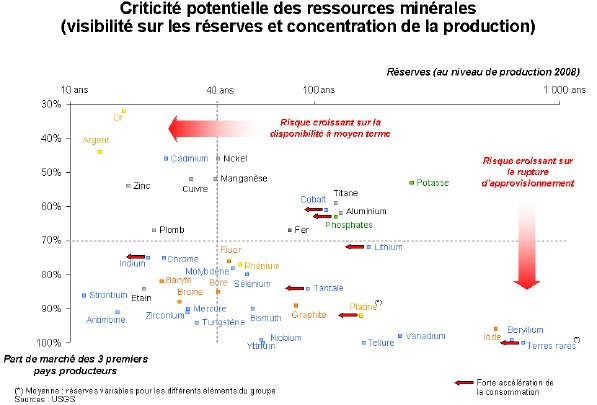
\includegraphics[scale=0.75]{./Rsc/risquemetaux.jpg}


On remarque que des métaux particulièrement importants tels que l'argent, le zinc ou le plomb sont considérés comme indisponibles d'ici 20 ans. Les pénuries de métaux auront un impact important sur de nombreuses industries.

\smallbreak Quelques organisations et états ont commencé à chercher des indicateurs de l'impact humain sur la planète.

La première est la dette écologique. D'après l'ONG Footprint Network la population vit à crédit depuis le 19 août cette année \cite{DateACredit}. Cette date correspond au jour où toutes les ressources consommées durant l'année sont trop importantes pour pouvoir être renouvelées. On vivrait ainsi "à crédit" à partir de cette date, portant une dette écologique. Le jour de ce dépassement était le 22 Septembre en 2003 et le 21 octobre en 1993.

L'empreinte écologique est un autre indicateur. Elle correspond à la pression exercée par l'homme sur la nature. On calcule le nombre d'hectare globaux (hag), c'est-à-dire une surface, dont une population a besoin pour générer ses ressources, puis les absorber. La valeur critique est de 1.8 hag. Si tout le monde avait cette empreinte, on utiliserait 100\% de notre planète. Pour un Français moyen, celle-ci est de 4.6 hag, ce qui signifie qu'il faudrait avoir 2.5 planètes pour absorber les déchets si toute la population mondiale était composée de Français. Les Américains ont besoin du double (9 hag).

\smallbreak Les ressources naturelles sont donc particulièrement demandées et certaines risquent de manquer dans les années à venir. De plus leur extraction est parfois dangeureuse et surtout polluante. L'\op est particulièrement liée à ce phénomène, puisque la fabrication de masse inhérente au modèle implique une forte demande toujours renouvelée. 

Cependant, l'extraction des matières premières n'est pas le seul danger pour l'environnement. En effet celles-ci sont ensuite transportées, transformées, lors de procédés parfois polluants.

%cite{LarousseMatiere1eres}

%cite{sociétéChimiqueDeFranceTerresRares}

%cite{RapportEuropeenTerresRares}

%cite{MongolieChine}

%cite{LivreFuturMetaux}

%cite{DateACredit}